% !TeX program = xelatex
\documentclass{hnie-thesis}
\usepackage{amsmath,amssymb,amsfonts,bm,mathtools}
\usepackage{graphicx}
\usepackage{booktabs,longtable,multirow,array,tabularx}
\usepackage{float}
\usepackage{algorithm}
\usepackage{algpseudocode}
\usepackage{listings}
\usepackage{xcolor}
\usepackage{hyperref}
\usepackage{enumitem}
\usepackage{caption}
\usepackage{subcaption}
\usepackage{setspace}
%\usepackage{titlesec}
\usepackage{fancyhdr}
\usepackage{makecell}
\usepackage{url}

\hypersetup{
    colorlinks=true,
    linkcolor=black,
    citecolor=black,
    urlcolor=black
}

\lstdefinestyle{pythonstyle}{
    language=Python,
    basicstyle=\ttfamily\small,
    keywordstyle=\color{blue!70!black},
    commentstyle=\color{green!40!black},
    stringstyle=\color{red!60!black},
    breaklines=true,
    frame=single,
    columns=fullflexible,
    showstringspaces=false
}
\lstset{style=pythonstyle}
\renewcommand{\lstlistingname}{代码}
\renewcommand{\lstlistlistingname}{代码清单}

\hniesetup{
  title={基于机器学习及车联网数据的\\车辆碰撞识别预警系统},
  english-title={Vehicle Collision Detection and Warning System based on Machine Learning and Vehicle-to-Everything Data},
  college={计算科学与电子学院},
  major={数据科学与大数据技术},
  class={大数据2101班},
  student-id={2021********},
  author={刘**},
  supervisor={文**},
  date={2025年6月2日}
}

\begin{document}

\makehniecover
\makehnieintegrity
\hniemaketoc

\hniebeginabstracts
\begin{cnabstract}
随着新能源电动汽车的飞速发展，各行业与用户对于低成本高效的车辆碰撞识别系统的需求越来越高。然而...

\hniekeywords{数据探索及清洗；特征工程；贪心随机网格搜索；随机森林；GBDT}
\end{cnabstract}

\begin{enabstract}
With the rapid development of new energy electric vehicles, there is an increasing demand across industries and among users for low-cost, high-efficiency vehicle collision detection systems. However ...

\hnieenkeywords{Data exploration and cleaning; Feature engineering; Greedy randomized search; Random forest; GBDT}
\end{enabstract}

\hniebodymatter

\chapter{绪论}

\section{引言}
为贯彻落实新发展理念、科技强国，国家大力推动新能源汽车的发展，电动汽车在国内占比逐渐增大。用户、汽车主机厂、保险等各行各业对于低成本、高效的新能源电动汽车的碰撞预警识别系统的需求越来越多。

然而...

\section{国内外研究现状}

\subsection{国内研究现状}
民用汽车从20世纪开始量产到如今已经成为现代社会重要的交通工具。截至2024年全国机动车保有量达4.53亿辆，其中汽车3.53亿辆，汽车产业成为国家经济系统的重要组成部分\cite{MinistryPublicSecurity2025MotorVehicles}。

在智能化...

\chapter{预备知识}

\section{特征编码}
非纯数字类型的定性特征字段可大致分为定类特征和定序特征两类，定类特征表明该记录所属类别，定序特征表明该记录在某指标下的某种程度，定类特征和定序特征常用的编码方式有两种，一种是直接用自然数进行编码的常规编码方式，另一种是独热指标（One-Hot Encoding）方式\cite{Yang2022SVMCostPrediction}。

...原理如图\ref{fig:one-hot}所示：

\begin{figure}[H] %H为当前位置，!htb为忽略美学标准，htbp为浮动图形
\centering %图片居中
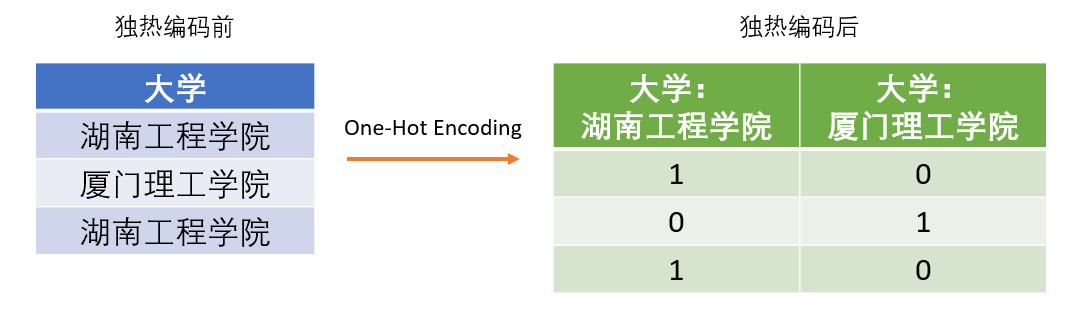
\includegraphics[width=\linewidth]{figures/image-20250519152157180.png} %插入图片，[]中设置图片大小，{}中是图片文件名
\caption{独热编码原理图} %最终文档中希望显示的图片标题
\label{fig:one-hot} %用于文内引用的标签
\end{figure} %结束环境

\section{重采样}

\section{分类模型评估方法}
...F1分数公式如下：
\begin{equation}
    \text{F1-score}=\frac{2\times \text{Precision}\times \text{Recall}}{\text{Precision}+\text{Recall}}.
\end{equation}

\chapter{数据预处理}
\section{数据探索及清洗}
\subsection{异常标签探索及清洗}
\subsection{缺失值及异常值探索及清洗}
...其中各个特征的缺失值数量如表\ref{tab:env}所示。

\begin{table}[H]
\centering
\caption{数据各特征缺失值数}
\label{tab:env}
\begin{tabular}{cc}
\toprule
特征名 & 缺失值数\\
\midrule
加速踏板位置 & 173443\\
驾驶员需求扭矩值 & 173321\\
电池包主负继电器状态 & 173321\\
电池包主正继电器状态 & 173321\\
制动踏板状态 & 173321\\
驾驶员离开提示 & 173321\\
主驾驶座占用状态 & 173420\\
驾驶员安全带状态 & 173321\\
手刹状态 & 173373\\
整车钥匙状态 & 173373\\
整车当前档位状态 & 173472\\
整车当前总电流 & 173373\\
整车当前总电压 & 173321\\
车辆行驶里程 & 173321\\
车速 & 173321\\
方向盘转角 & 173321\\
\bottomrule
\end{tabular}
\end{table}

本文的核心Pipeline框架如下：

\begin{lstlisting}[caption={基于Scikit-learn的Pipeline流程示例}]
from sklearn.compose import ColumnTransformer
from sklearn.impute import SimpleImputer
from sklearn.preprocessing import StandardScaler, OneHotEncoder
from sklearn.pipeline import Pipeline

numeric_transformer = Pipeline(steps=[
    ('imputer', SimpleImputer(strategy='median')),
    ('scaler', StandardScaler())
])
\end{lstlisting}

\hnieprintbibliography{references}

\begin{hnieacknowledgements}
本论文的完成离不开开源项目\cite{XurongLiu2026HNIETemplate}的支持，在此感谢项目作者 \textbf{XurongLiu} 的无私奉献。

...
\end{hnieacknowledgements}

\end{document}